% vim: ft=tex
\chapter{Approach}
This chapter describes the approach taken by the students to fulfill the
requirements. Possible variants as well as the final choices are explained here.

\section{Getting familiar with Roadster}
The client gave a short introduction into Roadster's code base during the meeting in the first
week of this thesis. Although quite overwhelming, the first impression was that
the code is clean, makes good use of abstractions and has loosely coupled
classes. API documentation is scarce though.

TODO: describe approach of getting more familiar with Roadster, e.g. during prototyping

\section{Testing}
This section describes the test methods we used to check particular methods,
the integration of multiple components, as well as the behavior of the whole application.
All test resuts can be found in \autoref{ch:res}.

\subsection{Setup}
Due to the fact that Roadster's Github repository is private, online \gls{CI}
services such as \emph{Travis
CI}\footnote{url{https://travis-ci.com/}} can't be used without
payment\footnote{Payment is required after the first 100 builds.}. Fortunately,
Gitlab CI is free and can be installed on one's own infrastructure, such as the
\gls{VM} provided by HSR, where it was installed and configured. Unit and
integration tests are run every time new commits are checked in. This is useful
to get informed proactively when something breaks.

\subsection{Unit tests}
To ensure the correctness of the implementations, unit tests are written using
RSpec. 100\% coverage of the students' contributions can be achieved by
adhering to \gls{TDD}. Naturally, this also simplifies refactoring the code
without risking things breaking silently. Unit tests reside under the \sh{spec}
directory of Roadster's code base.

\subsection{Integration tests}
Integration tests verify the interaction between the individual components.
To test core features like federation, high availability, and persistence
synchronization, integration tests have been written. Multiple nodes can be
simulated easily by starting them as different process groups. This is possible
since \zmq completely abstracts the transport away.

In order to test the failover or synchronization functionality, individual processes
can simply be killed and restarted later if the scenario defines this.

More details about the integration test scenarios can be found in \autoref{ch:res}.

\subsection{Continous integration}
\gls{CI} helps us prevent integration problems also known as \emph{integration
hell}. Each push to the repository will trigger a CI build using a predefined
build script. This will install Roadster's dependencies, an example app built
with Roadster, and run finally Roadster's test suites.

\subsection{System test}
System tests are designed to test the application under close-to-reality conditions.
To create a realistic environment, Mininet and fake \glspl{PLC} are used.
\begin{description}
	\item [Mininet:]\hfill\\
		Mininet allows creating virtual networks instantaneously. It
		relies on Linux cgroups and network namespaces to isolate the
		\glspl{VM}, the very same primitives used by Docker.
		Mininet can also simulate link/connectivity problems between nodes.
	\item [Fake:]\hfill\\
		Fake \glspl{PLC} are simple scripts that respond to requests.
\end{description}

All events are stored in log files which are subsequently used for the
evaluation of the test result.  A Ruby program checks these log files for
correctness. All system tests are performed manually after each construction
iteration.

\subsubsection{Test scenarios}
The test scenarios primarily test situations encountered in the real world. Out
of scientific interest, more test scenarios, which reflect more extreme cases,
have been added.
% TODO: mention the Gherkin features

The test scenarios contain configurations for mininet and the particular Roadster nodes.
The procedure of each scenario is described in detail below to make the results reproducible.

% TODO work out methodology (maybe with mininet, shell scripts, and analyze logs retrospectively)
% TODO integration tests at the end of every iteration
% TODO system tests at end of construction
% TODO setup GitLab CI (self-hosted on HSR VM)

%----------------------------------------------------------------------------
\section{Port to new \zmq library}\label{sec:approach:port}
Porting Roadster to a new \zmq library early on makes sense for the following reasons:

\begin{itemize}
\item to exclude possible failures from faults in the unmaintained ffi-rzmq\footnote{\url{https://github.com/chuckremes/ffi-rzmq}} library
\item encryption is needed later anyway, which is not supported by the currently used library
\item all other tasks involve \zmq communication anyway
\end{itemize}

There is currently only a single Ruby library that is maintained, supports
encryption, and freely available, which is \gls{cztop}. Technically it's a
binding for the \gls{czmq} library, which is the modern and recommended way of
using \zmq. More info about CZMQ can be found in \autoref{ch:zmq}.

As stated in the Task Description already, Roadster's event loop makes use of
the \zmq options \sh{ZMQ_FD} and \sh{ZMQ_EVENTS}. Getters for these had to be
added to in CZTop, which was a matter of minutes.

\subsection{Actual port}
Due to Roadster's beautiful software architecture, code that actually made use
of the ffi-rzmq library directly was located in a single file. The following
things needed to be done:

\begin{itemize}
\item Tell Ruby to load CZTop instead of ffi-rzmq.
\item Remove code to manually send and receive the parts of multi-part messages. This has been simplified
in CZMQ and thus is a single method call using CZTop.
\item Remove error checking code. CZTop always checks error codes, and raises
an appropriate exception if needed.
\item Simplify code that reads option values such as \sh{ZMQ_FD} and \sh{ZMQ_EVENTS}.
\item Rewrite library calls to use CZTop instead of ffi-rzmq.
\end{itemize}

This was about an hour's work.

%----------------------------------------------------------------------------
\section{Federation}\label{sec:approach:federation}
A Roadster federation is illustrated in \autoref{fig:federation}. Adding federation
functionality to Roadster involves the following aspects:
\begin{itemize}
	\item node topology DSL

		This DSL also has to provide means to define the
		roles/functionality of each node, e.g. the set of COMM actors
		running on a particular node

	\item DIM synchronization
	\item message routing
	\item What needs to be done if a WebUI user wants to e.g. change some
		value on a PLC, possibly on a remote node? Is it completely
		handled via DIM or do we need message routing?
\end{itemize}

\begin{figure}[]
	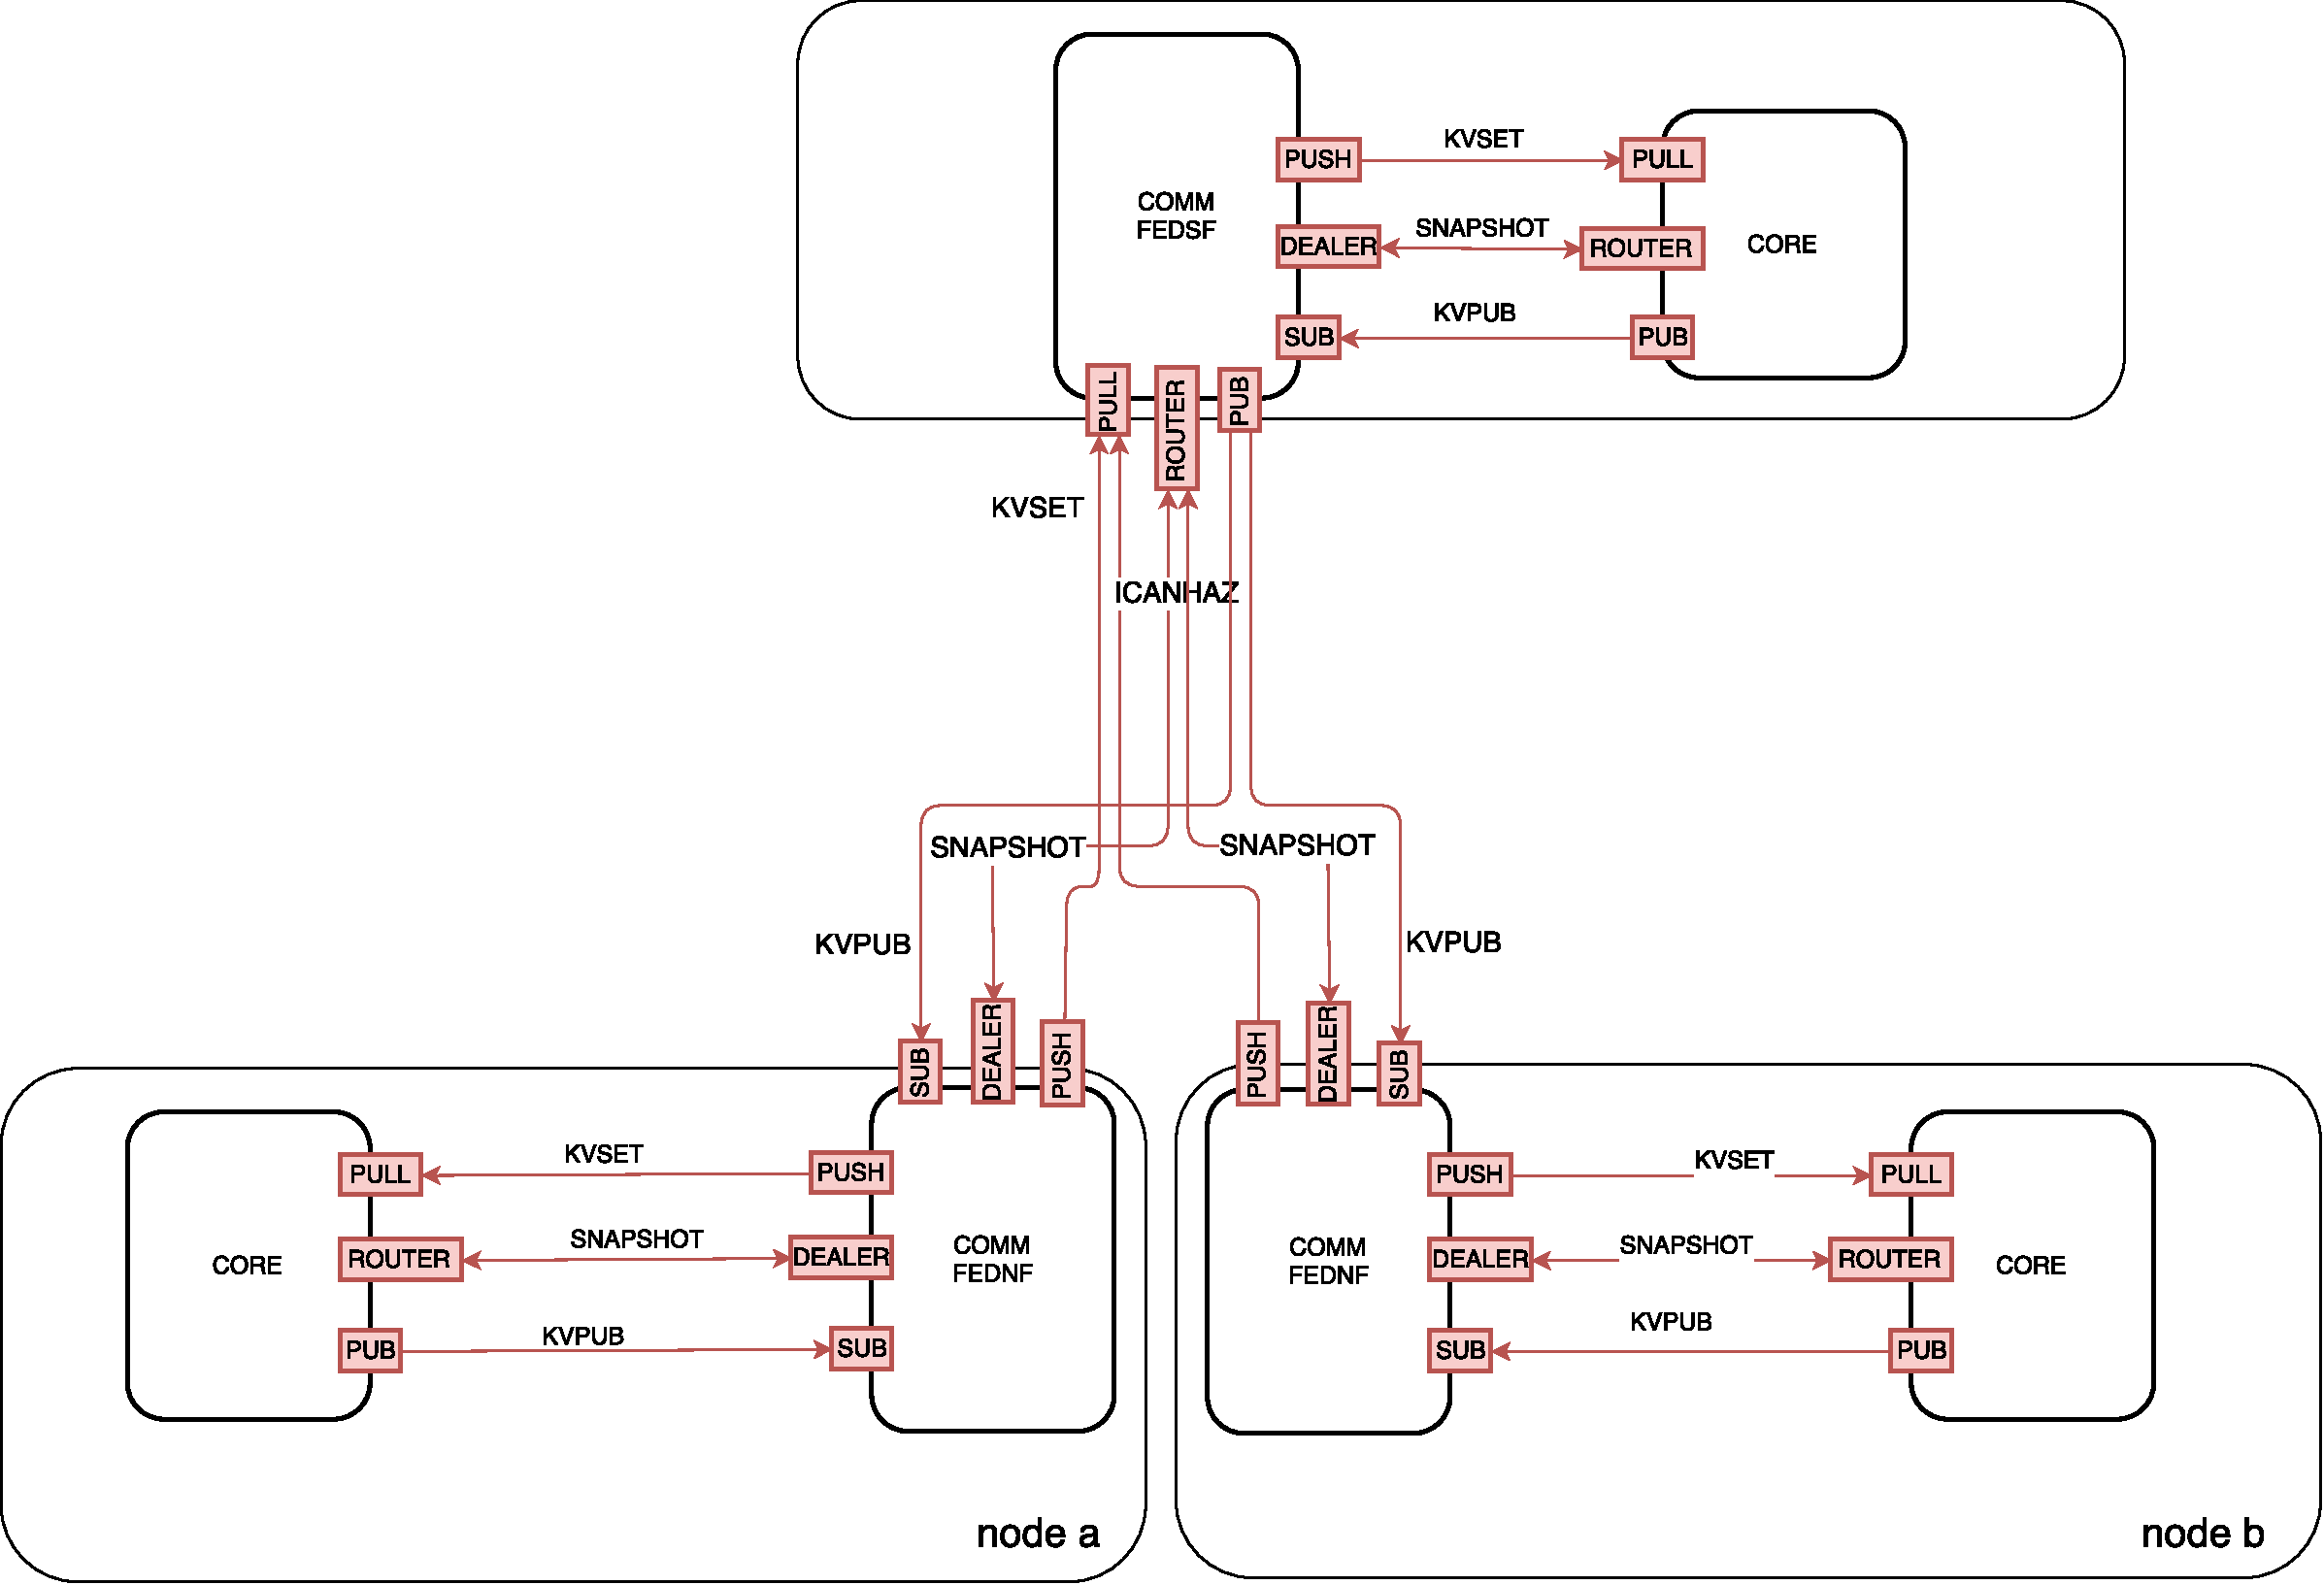
\includegraphics[width=\textwidth]{img/federation_protocol.pdf}
	\caption{Federation between a supernode and two subnodes}
	\label{fig:federation}
\end{figure}

\subsection{DIM synchronization}
DIM synchronization has to work across a hierarchical federation of nodes. It
also needs to be able to handle HA clusters.

\subsubsection{New COMM actors}
Since COMM actors are used to communicate with things outside of a node, new COMM
actors will have to be introduced: One kind that is north-facing to communicate
with subnodes, and another one that is south-facing for communication with the
supernode. They will be named COMM FEDNF and COMM FEDSF. These names have been
chosen because they're unambiguous. Names such as "north" or "upstream" would
be ambiguous. Is it the actor residing in the northern communication partner?
Or is it the one communicating with the northern partner? "Upstream" would be
even more confusing, as in the open source world it commonly refers to the
mainline developed by the official authors, i.e. the source of truth. There's
no concept within Roadster unambiguously corresponding to this meaning. So the
benefit of choosing names that imply an actor is north-facing or south-facing
is clarity.

The new actors' responsibility is the inter-node synchronization of the DIM,
similarly to what's happening in the existing \gls{CSP} within a single node.
To do so, they simply subscribe to DIM updates within a node just like any
other actor does.  Then they replicate any subsequent updates over the network
to the neighbors (supernode, and subnodes).

% TODO: describe FEDSF and FEDNF

\paragraph{CAP theorem}
The CAP theorem \cite{wp:cap} states that it is impossible for a distributed
computer system to simultaneously provide consistency, availability, and
network partition tolerance. In the face of a network partition, one has to
chose between availability and consistency. Because subsystems of a Roadster
federation must be autonomous, the obvious choice is availability.

Eventual consistency is guaranteed by restricting write access to the owning
node, and recovering from a network partition when communication is restored is
done by simply reinitiating the DIM synchronization process.

\subsubsection{Object ownership}
The concept of ownership has to be introduced. Every object within the DIM
shall belong to a single node. Modifications to the objects shall be done via
that node, so the node is the source of truth for all modifications for the
objects it owns. For that, every object in the DIM has to have a referennce
(i.e. an attribute \rb{@owner}) to the object representing its owner node, which is part of
the configuration that is loaded from the static configuration loaded by every
actor at initialization.

\subsubsection{Degree of synchronization}
There are multiple choices when it comes to what exactly of the DIM should be synchronized:

\begin{description}
	\item [Variant 1. Sync self-subtree only] \hfill\\
	Always sync on subtree only, which means a node only knows the DIM part of
	itself. The big disadvantage is that it won't have a copy of the rest of the
	DIM, which can be useful to inspect variables on neighboring nodes, especially
	when they're unreachable.

	\item [Variant 2. Sync complete tree] \hfill\\
	Always sync on complete tree, which means getting the snapshot from the
	supernode and merge the own subtree into it, replacing whatever subtree is
	already there. This works because of the autonomy requirement for nodes and
	their subnodes. This variant is very easy to implement at first.

	\item [Variant 3. Either sync on subtree or complete tree] \hfill\\
	Make it configurable: Either sync on subtree or on complete tree. The
	toplogy DSL would allow to specify this property for each node. This is
	the best of both worlds, but more effort.
\end{description}

Variant 2 will be the first step, as following the \gls{KISS} principle is one
of the non-functional requirements. Variant 3 will be the second step, if at
all. This depends on whether it'll be needed performance-wise.

\subsection{Node topology definition}
The federation topology has to be defined somewhere. This can be done using a
\gls{DSL} and then put into a static file (e.g. \sh{topology_conf.rb}) shared
on all nodes of a Roadster federation. Each actor could then read the file at
startup, just like it's done for other configuration pieces of a Roadster node.
\autoref{lst:dsl:topo:no-ha} shows how such a configuration snippet might look.

To let the actors of a node know which node they belong to, an additoinal line
has to be added to the specific configuration file (\sh{conf.rb}), e.g.
\rb{conf.system_id = "nodes.root"}. Using that information, the topology
created using the DSL can be walked like a tree to find the correct node and
important information like its neighbor nodes.

A HA node pair could be one DIM object which has one name but two IP addresses
(primary and backup, in that order). Direct subnodes can use that information
to connect to the correct supernode during normal operation and also
when the primary node is unavailable. The respective DSL snippet is shown in
\autoref{lst:dsl:topo:with-ha}.

Not every node in a federation has the same role: Some are only connected with other
nodes, some directly communicate with field devices. To define different node roles, a
syntax as shown in \autoref{lst:dsl:topo:with-roles} is possible.

\begin{listing}
	\caption{Federation DSL example without HA}
	\label{lst:dsl:topo:no-ha}
	\begin{minted}[bgcolor=bg]{Ruby}
# * basic method to add a node: #add_node(ID, south_facing_bind_endpoint)
# * it takes a block for defining subnodes

conf.nodes do |map|
  map.add_node("root", "tcp://10.0.0.1:5000") do |map|
    map.add_node("subnode_a", "tcp://10.0.0.10:5000")
    map.add_node("subnode_b", "tcp://10.0.0.11:5000")
  end
end

# subnode_a can infer its endpoints from its position in the tree:
conf.system_id = "nodes.root.subnode_a"
#=> this node is "subnode_a"
#=> its IP address is 10.0.0.10
#=> north facing COMM actor's bind port is 5001
#=> south facing COMM actor's bind port is 5000
#=> north facing COMM actor will connect to "root" node on "tcp://10.0.0.1:5000"
	\end{minted}
\end{listing}

\begin{listing}
	\caption{Fedreation DSL example with HA}
	\label{lst:dsl:topo:with-ha}
	\begin{minted}[bgcolor=bg]{Ruby}
conf.nodes do |map|
  map.add_ha_pair("root", "tcp://10.0.0.1:5000", "tcp://10.0.0.2:5000") do |map|
    map.add_node("subnode_a", "tcp://10.0.0.10:5000")
    map.add_node("subnode_b", "tcp://10.0.0.11:5000")
  end
end

# subnodeA can infer its endpoints from its position in the tree:
conf.system_id = "nodes.root.subnode_a"
#=> this node is "subnode_a"
#=> its IP address is 10.0.0.10
#=> north facing COMM actor's bind port is 5001
#=> south facing COMM actor's bind port is 5000
#=> north facing COMM actor will connect to "root" HA pair on "tcp://10.0.0.1:5000" OR "tcp://10.0.0.2:5000" (Lazy Pirate algorithm)

# for primary root:
conf.system_id = "nodes.root[primary]"
	\end{minted}
\end{listing}

% ############
% # within ba-roadster-app's lib/domain/domain.rb file:
% #
\begin{listing}
	\caption{Federation DSL example with HA and roles}
	\label{lst:dsl:topo:with-roles}
	\begin{minted}[bgcolor=bg]{Ruby}
# Idea for node topology definition and assigning roles (features/adapters) to
# diffent kinds of nodes.

module Roadster
  module Domain::Model

    build do
      nodes do
        node "root" do # or maybe ha_node or bstar_node
          endpoint "tcp://10.0.0.1:5000", "tcp://10.0.0.2:5000"
          label 'BA Roadster App'
          desc  'Sample application for experimenting and developing the new features within the scope of the Bacherlor Thesis of Patrik Wenger and Manuel Schuler at HSR.'

          load_conf ::Conf::AccessControl
          load_conf ::Conf::Objects
          load_conf ::Conf::Navigation

          node "subnode_a" do
            endpoint "tcp://10.0.0.1:5000"
            load_conf ::Conf::Adapters
            # load_conf ...
          end
        end
    end

  end # Domain::Model
end # Roadster
	\end{minted}
\end{listing}


\subsection{Message routing}
Messages need to be sent from an actor on one node to an actor on another node.
The best place to put this logic is the CORE actor which already does this for
messages exchanged within a node. It needs to be extended to know about nodes
and their actors, not only actors on the current node. Then messages can be
passed around hop-by-hop.

In case a message is sent in \emph{Dialog} mode, this implicates Russian doll
routing: At every hop, a new dialog is started which expects an immediate
response, which will subsequently be passed back and complete the open dialogs.

\subsubsection{Example}
When a user of the root node's web UI wants to change a value on a field device
connected to the root node's subordinate node, a command is sent from the
browser to the web UI's COMM actor. From there it's sent via the CORE actor out
on the FEDSF actor to the subordinate node. There it's routed
via the CORE actor to the correct COMM actor, where the command can actually be
executed on the field device.

%----------------------------------------------------------------------------
\section{High availability}\label{sec:approach:ha}
% TODO: HA node => HA peer, backup node => backup peer (??), active peer, passive peer?
% TODO: diagonal HA
% TODO: with OPC UA in mind
% TODO describe possible scenarios where failover will work/not work
%       - as complete as possible
%       - maybe gherkin style
%       - dedicated link is possible, typically not
If Roadster is going to be run in a federation, measures need to be taken to
mitigate the risk of failure, since many nodes are more likely to fail than a
single node (unless they add redundancy). Availability shall be ensured by
adding redundancy on certain levels of the node hierarchy (e.g. at the bottom
of the topology, right above the PLC, or at the root level), in the form of a
fully functional backup node in addition to the primary one.

Run together in a hot-standby cluster, the passive node's responsibility is to
take over in case the active one goes down.

\subsection{Defining reliability}
When speaking about reliability, it's worth listing the failures we want to be % FIXME
able to handle. According to the requirements, these are exactly:

\begin{description}
	\item [Hardware or software failure on the primary node:]
		This could be one of the actors crashing, the whole OS
		crashing, or a fatal disk failure, irrecoverable memory error,
		or even just someone accidentally pulling the power plug.
		% TODO: more detailed

	\item [Network failure]
		This only includes the failure of the link connecting a HA node
		to the rest of the federation.  Interestingly, this limitation applies to both
		single level and multi level HA.
		% TODO: more detailed
\end{description}

Failures that won't be covered include:
\begin{description}
	\item [Failure of the link between a subnode and one of its supernodes:]

		This can't be handled since the two HA peers would have to
		continually share the number of subnodes connected to them, and
		based on that, make a decision on which one should be active or
		passive. Since the link between them could fail as well, this
		decision can't be done reliably, which could lead to the
		dreaded split brain syndrome.
		% TODO: this protocol extension should be possible, communicate
		% number of fully synchronized clients, if it stays 0 for 3
		% cycles & ICANHAZ requests are coming, backup shall take over


	\item [Failure of the link between a HA peer and the field device]
		The \gls{bstar} algorithm won't initiate a failover since the
		active is still alive and is able to tell the passive node so.
		The missing life signs via the field device could cause an alarm, but no
		failover, since they're only half of the conditions that have
		to be met for a failover.
		% TODO: more detailed
\end{description}

The \gls{zguide} describes a very simple mechanism to achieve this kind of high
availability with exactly two redundant nodes: The \gls{bstar}. It
provides a set of clients a highly available service by running two server
nodes in a hot-standby setup. It is simple and thus very robust, avoids the
split-brain syndrome, and is fairly easy to implement, even as reusable
code. The implementation could be contained within a new kind of COMM actor
called BSTAR. This makes sense since it talks to the outside world.

% TODO maybe we need to extend binary star to handle other kinds of network failures?

\subsection{Binary Star in a nutshell}
Two HA peers are started either as primary or as backup. After an initial
handshake, the primary one becomes active, the backup node becomes passive. The
two continually exchange heartbeats. Clients always connect to the primary's endpoint first.

The passive node takes over when the following two conditions are met:

\begin{enumerate}
\item no life signs from the active node
\item connection requests from clients
\end{enumerate}

The second condition is to prevent the split-brain syndrome and thus can be
thought of as an external vote for the node to actually initiate the failover.
This works because clients will always try to connect to the primary node's
endpoint first, then move on to the backup node's endpoint. This algorithm is
explained in \cite[Chapter 4 - Reliable Request-Reply Patterns, Client-Side
Reliability (Lazy Pirate Pattern)]{zmq:zguide}.

\subsection{Failover}
In case the currently active peer goes down, the two conditions will be met.
This means that the passive node starts accepting snapshot requests (ICANHAZ
messages) and updates the DIM, so every other node will know about the new,
active node. This is needed for the message routing to work.

% TODO: move down?
It's important to mention that a dedicated, direct link from one HA node to its
peer actually worsens high availability. In case the non-dedicated link from
the primary HA node goes down, meaning the HA node is effectively offline and
unavailable for subnodes, the failover won't happen since heartbeats are still
exchanged with the HA peer over the dedicated link.

% TODO No client => no failover

\subsubsection{Alarm generation}
When a failover happens, it makes sense to create a \rb{Case} (alarm) in the
DIM, so the outage is visible to operational personnel in one of the web UIs.
The same applies to the case where the passive node goes down, although it
doesn't have an immediate effect on availability.  This is so the operational
personnel can act upon the alarm and e.g. initiate field forces to inspect the
failed node and repair it.

Once repaired, it's restarted with the exact same configuration --- either primary
or backup. Since there's already an active node (either the primary one,
or the backup one), the newly repaired node will become the new passive node.

\subsubsection{Failover from backup to primary node}
Once failed over, the newly actve backup node stays active. It does so until it
fails itself or is manually stopped. It never automatically switches back to
make the primary node the new active one without a failure. This is key. If a
node becomes unreachable, the failover happens automatically, but anything else will
require human interaction.

Subsequently, when the previously broken, primary node has been repaired, it
rejoins the \gls{bstar} cluster as the passive node. At that point, the backup
node can be killed if need be, and the primary node will take over again.  This
works because the \gls{bstar} operates symmetrically after a successful
handshake during initialization.

\subsection{Side benefit: Rolling upgrades}
% TODO useful for upgrades (maybe in Discussion)

\subsection{A note on dedicated links}
The \gls{zguide} mentions that a dedicated link between the two HA peers
(traditionally done with a crossover cable) is the best solution to prevent the
split-brain syndrome. This is true. But in some cases, it could also prevent a
failover from happening.

Imagine the currently active peer's other network equipment fails, i.e. its NIC
connected to the switch fails, or its switch port fails, then it's unreachable
to the rest of the federation. In that case, a failover would be wanted. But it
can't happen, since heartbeats are still exchanged with the passive node over
the dedicated link. So it's a trade-off between risking the split-brain
syndrome and not being able to perform a failover.

\subsubsection{Extending \gls{bstar}}
Of course the \gls{bstar} mechanism could be extended to
communicate the number of fully connected clients. That way, a passive node
could recognize the situation correctly, since it will get requests from
clients which are trying to fallback to it since the active peer is
unreachable. Knowing its active peer has zero connected clients, it could
actually promote itself to the new active peer.

For this to work, a way of counting fully connected (not just requesting)
clients has to be introduced. Since \zmq abstracts connection handling
completely away, this needs to be done using heartbeats, i.e. from the clients
that are currently fully connected (i.e. registered to receive DIM updates).
This number, or list of clients, could be communicated privately just between
the two HA peers, along with the heartbeats, or it could be published via the
DIM.

Another thing that's needed is a HA peer's ability to step down from being the
active node as soon as its peer promotes itself to the newly active peer. In
the standard \gls{bstar} mechanism, this would be recognized as the split-brain
syndrome and handled fatally.


\subsubsection{Dangerous corner case}
% TODO Backup node active, dedicated link goes down, and there are new/reconnecting clients}
% TODO this will lead to split-brain syndrome (maybe in Discussion)
% TODO in general: dedicated link for HA pair communication is dangerous!

\subsection{Single level}
This is different from what's described in the \gls{zguide} because the concept of
client requests is missing here (field devices don't request anything from Roadster nodes).  What can be
done instead is periodically sending life signs from one node to the other
through the field device by updating some designated memory block. This can actually be
done by both the active and the passive node, which reduces code complexity.

The passive node will check the active node's life signs periodically as well.
In case the life signs cease, it can give its vote to the COMM BSTAR actor.
This would satisfy the second condition of the \gls{bstar} for a
failover to take place. The first condition would be the missing heartbeats
which are normally transmitted through the network link.

TODO new actor: COMM BSTARVOTER (or maybe directly into CORE actor)

\begin{figure}[]
	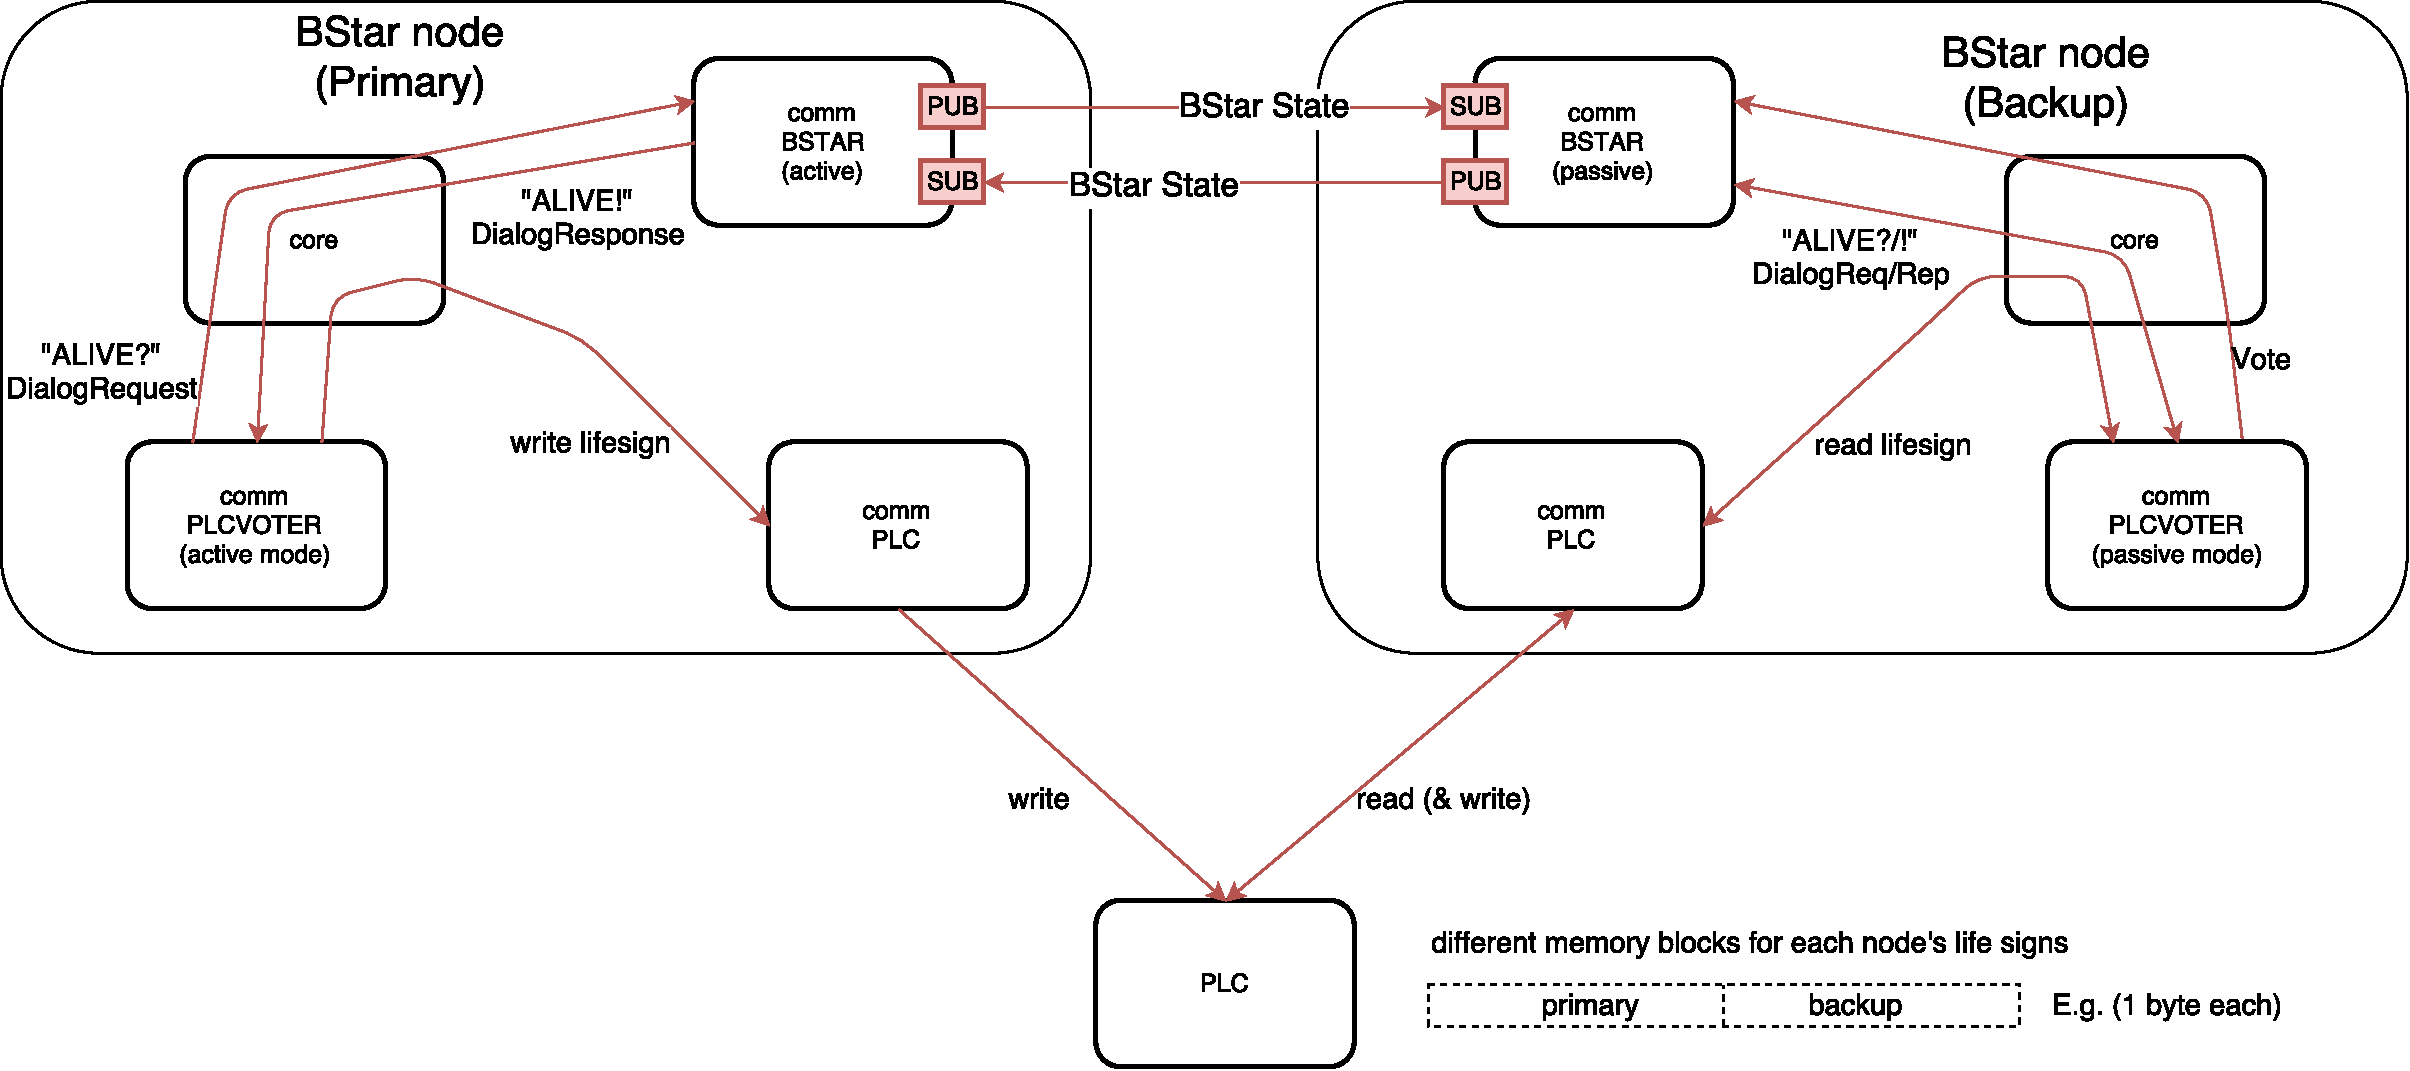
\includegraphics[width=\textwidth]{img/SL-HA_bstar.pdf}
	\caption{Single level HA setup between a HA pair and a field device (PLC)}
	\label{fig:sl-ha}
\end{figure}
% TODO: mention figure in text

\subsubsection{Caveats}
Special attention needs to be paid when it comes to writing these life signs. A
na\"ive developer might implement the COMM BSTARVOTER so it autonomously causes
life signs to be written on the field device. This works as long as the failures only affect
the hardware. But what if a software error happens in the CORE or BSTAR actor?
They'd crash or hang, while the BSTARVOTER happily sends out life signs, which it
obviously shouldn't be doing at that moment.

A better implementation would have the BSTARVOTER poll the BSTAR via the CORE
router whether it's still alive, and only send out a life sign in case it gets
an answer. This way, the BSTAR and the CORE actor are being tested for
responsiveness. We'll call the two messages being sent back and forth "DEAD?"
and "ALIVE!".

\subsubsection{Link failure between Roadster node and field device}
TODO describe why this won't cause a failover and thus can't be handled, as
mentioned above\\

\subsubsection{Supporting different field devices}
TODO: adapter

\subsection{Multi Level}
This kind of \gls{HA} setup is closely related to the \gls{bstar} described
in \cite[Chapter 4 - Reliable Request-Reply Patterns, High-Availability Pair
(Binary Star Pattern)]{zmq:zguide}. This means that the passive node would
actually receive requests from clients in case the active node fails, which
simplifies the implementation. These requests will count as votes to fulfill
the second condition that has to be met for a failover to be initiated. This is
illustrated in \autoref{fig:ml:ha}.

\begin{figure}[]
	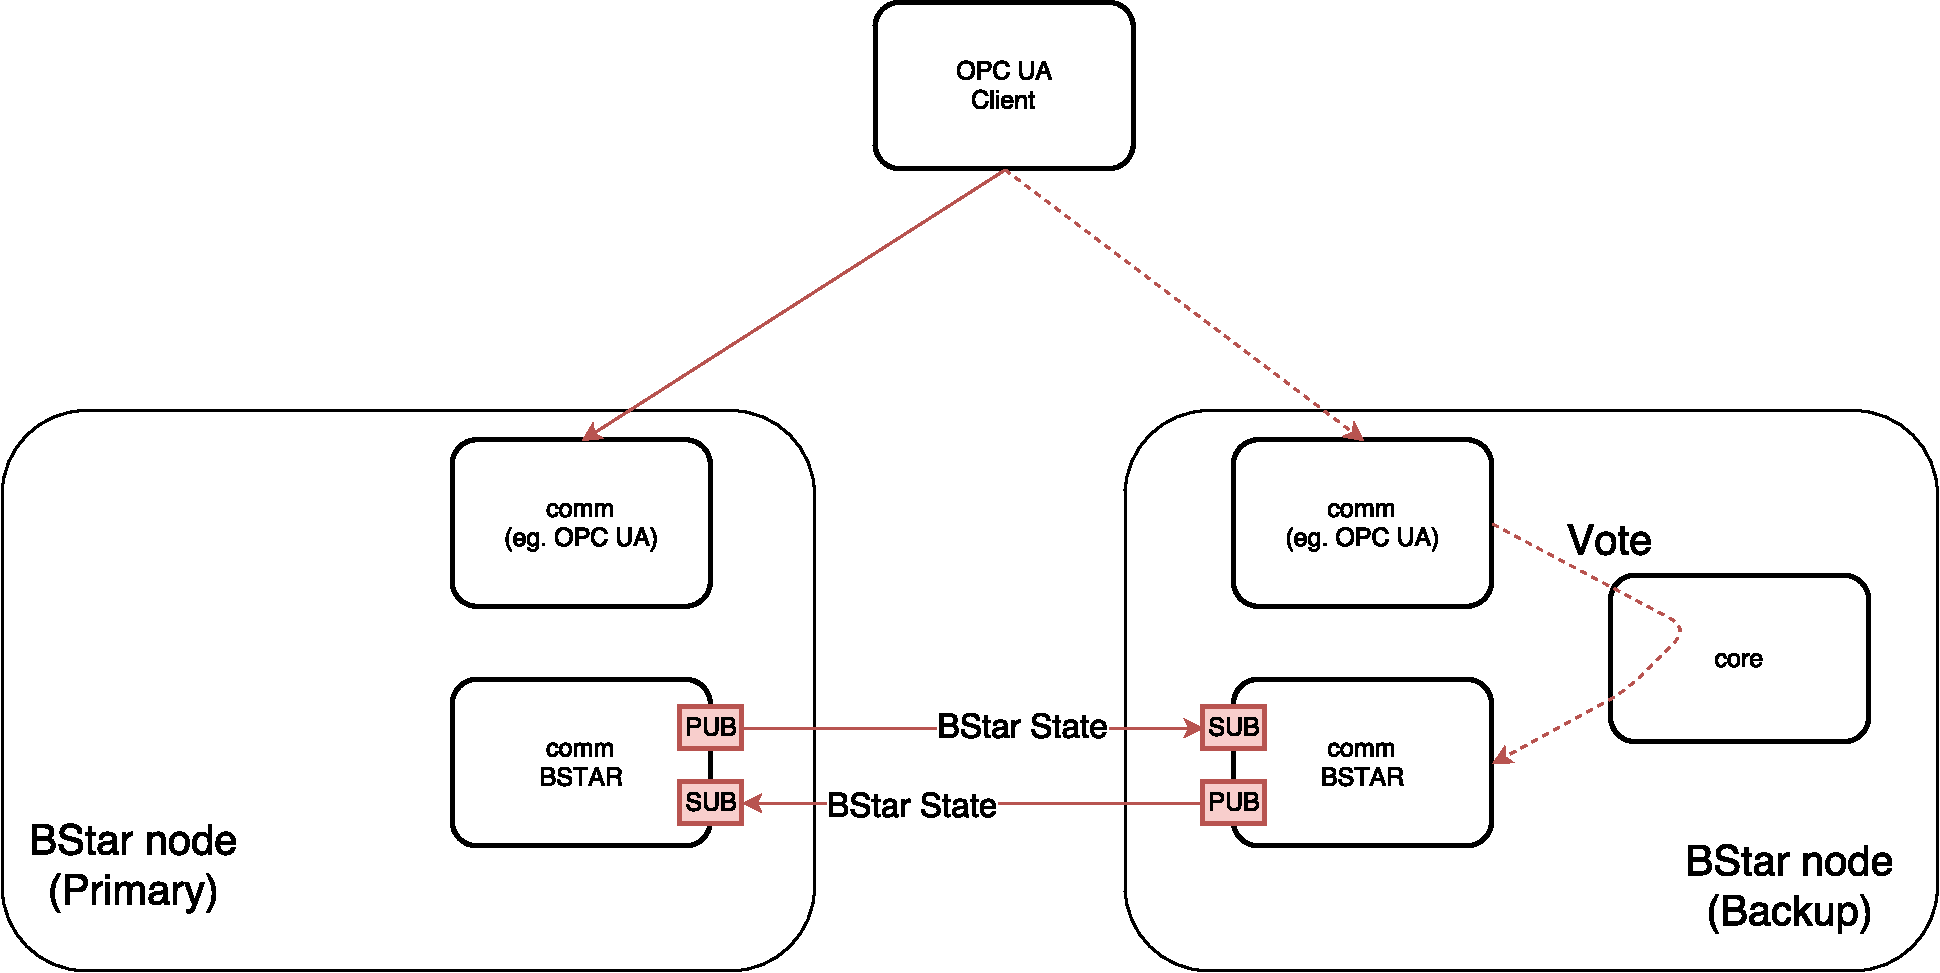
\includegraphics[width=\textwidth]{img/ML-HA_bstar.pdf}
	\caption{Multi level HA setup between a HA pair and a number of client nodes}
	\label{fig:ml:ha}
\end{figure}

%----------------------------------------------------------------------------
\section{Persistence synchronization}\label{sec:approach:psync}
The persisted data and updates to it, handled by the STORAGE actor, need to
bubble up and collected in the root node.

\subsection{Aspects}
There are multiple aspects involved in persistence synchronization:

\begin{description}
	\item [Initial synchronization:]
		How does one get the initial delta of updates since the last
		synchronization?

	\item [Continuous synchronization:]
		Further updates, one-by-one. This is only needed in
		case the solution aims for event-driven (meaning close to
		instantaneous) synchronization.

	\item [HA peer sync:]
		How is the passive HA peer updated?
		This not only matters when the supernode is a HA pair (multi
		level), but also when it's at the bottom of the node hieararchy
		(single level).

		% TODO
		\large\color{red} What about that last case? We need to synchronize
		east-west. Something similar as with Binary Star, where updates
		go into a \emph{pending} queue on the passive node until
		confirmed by the active node?
\end{description}

% TODO: how to find out delta?
% - event journal: request oldest non-finished case from owner
% - time series: north-traffic only, bubble DELETESs
% - parameters: every param is also owned by some node, user passwords are owned by root

\subsection{Variants}
There are multiple variants to achieve the needed functionality.
% NOTE: Client seems to favor polling.

\subsubsection{Polling only}
The supernode just periodically request persistence
deltas. This would be handled over a DEALER/ROUTER pair of sockets. The nice
thing about this variant is that the subnode only has to do one thing, which is
responding to requests from the supernode(s); it doesn't have to proactively
send any updates after sending the an initial delta.

A big drawback is that the synchronization only happens periodically. This
doesn't seem to fit well into the overall Roadster architecture, which is
completely event-driven (no polls or "sleeps").

Another drawback is efficiency. This variant will periodically cause the
subnode's database to be searched for all keys. Depending on the size of the
database and the efficiency of searching through keys, this could be a lot of
wasted resources or even cause bottle necks when interacting with the STOR
actor.

In case the supernode is a HA pair, this variant would generate duplicated
traffic. To avoid this, another pair of sockets has to be introduced to
synchronize persistence between a HA pair. This also means designing another
protocol, and more moving parts overall.

% TODO: SL-HA

Overall, this variant is very simple, but doesn't offer some features we'd
normally expect from a framework like Roadster. The fruits are hanging low;
achieving event-driven synchronization and better efficiency is easy.

\subsubsection{PUSH-PULL}
This variant avoids the delays introduced by the polling mechanism of the first variant.

Procedure (for each subnode):
\begin{enumerate}
	\item via a ROUTER/DEALER socket pair:
		\begin{enumerate}
			\item supernode tells subnode its most recent timestamp in an ICANHAZ request
			\item subnode sends delta
			\item supernode receives and processes the complete delta
		\end{enumerate}
	\item subnode sends updates to supernode via PUSH-PULL
	\item during low-traffic times, we can send HUGZ as heartbeats
\end{enumerate}

This seems nice at first, but the PUSH socket's send buffer will fill up when the
connection is interrupted.  This isn't bad in and of itself, because when it's
full (and writes start to block), we can just destroy the socket and
reinitialize and start syncing anew (from ICANHAZ) after a certain timeout.
But the problem is that, in case the delta is large, it will inevitably fill
the PUSH socket's send buffer, temporarily reaching its high water mark, which
is part of its normal operation.

So we'd have to introduce logic to recognize whether the PUSH
socket is just temporarily full (e.g. during delta transmission), or
permanently full (e.g. the supernode or the link to it is down).

% TODO: SL-HA

Another disadvantage is that there needs to be another channel to synchronize
persistence updates to the other HA peer, if there is one. This means another
pair of sockets, another protocol to be designed, and more moving parts
overall.

\subsubsection{PUB/SUB}
This is similar to \gls{CSP}/\gls{CHP}. It's not 100\% reliable, but even with unstable
links, no data loss will occur if the client (the supernode) is able to reconnect within a
specific amount of time. \zmq's default for that amount is 10 seconds. As the
requirements specify, 100\% consistency is not mandatory for the persistent
data.

A possible drawback is that the traffic is duplicated in case the supernode
is a HA pair. However, there are numerous opportunities to mitigate this.

Procedure (for each subnode):
\begin{enumerate}
	\item supernode subscribes to updates from subnode
	\item via a ROUTER/DEALER socket pair:
		\begin{enumerate}
			\item supernode tells subnode its most recent timestamp in an ICANHAZ request
			\item subnode sends delta
			\item supernode receives and processes the complete delta
		\end{enumerate}
	\item supernode starts reading updates, possibly skipping the first few (based on timestamp)
\end{enumerate}

% TODO: SL-HA

\subsection{Chosen Variant}
We'll most likely go with the PUB-SUB variant, since it's simple and is similar to
what's used for the new \gls{CSP} in conjunction with multi-node \gls{HA}. It provides the best
opportunities to improve efficiency later on.

Its possible performance issues can be ignored right now, as trying to fix them
is arguably considered premature optimization. If this turns out to be an issue
in a productive deployment, like over a cellular network link, a future version
can switch to multicast. \zmq supports PGM, which is a reliable multicast
protocol. (Pragmatic General Multicast, standardized, directly on top of IP,
requires access to raw sockets and thus may require additional privileges) and
EPGM (Encapsulated Pragmatic General Multicast, encapsulated in a series of UDP
datagrams, doesn't require additional privileges, useful in a \zmq-only setup).

If its reliablity turn out to be an issue, one the socket option
\sh{ZMQ_RECOVERY_IVL} can be increased from 10 seconds to, say, 60 seconds, which
gives an unstable link more time to recover before any data loss happens.

TODO: describe reasonable default setting, in case we change ZMQ's default.


\section{Encryption}\label{sec:approach:encryption}
It's fairly easy to enable transport security to secure the communication
between \zmq sockets over an unsecure network.

\subsection{Assigning socket roles}
Because \zmq allows any order of the bind and connect actions to take place,
and doesn't impose a specific action on each socket type, the meaning of
"server" and "client" become blurry. Still, with respect to the CURVE security
mechanism in \zmq, one of the two involved sockets needs to be designated as
the CURVE server, and the other one as a CURVE client.\footnote{This is a
simple method call on each socket where the involved keys are passed as well.}

Based on the autonomy aspect of the federation, meaning the lower-level systems
act as servers for the higher-level systems, it would have been neat to follow
the same schema for the roles of the CURVE server and client. Unfortunately
that's not possible, because the a CURVE client socket is assigned exactly one
CURVE server certificate. But in a tree, the supernode can have multiple
subnodes. Thus, the socket inside supernode's FEDSF actor will be designated as
the CURVE server, and the sockets inside the subnodes' FEDNF actors will be
designated as the CURVE clients.

\subsection{Mutual authentication}
% keys on both sides, and which nodes need whose public key
In addition to the server authentication, which is always performed, client
side authentification is desired. This means that each federation node must be
in possession of its respective clients' public keys. Since CURVE servers are
on the south-side of each inter-node connection, and every node in a
hierarchical tree has at most one supernode, that means storing exactly one
client public key on affected nodes. A special case are subnodes of HA
clusters. There it'd be two client public keys (unless both HA peers share the
same key pair, which is not recommended).

% distribution of public keys
Public keys and the private keys are generated in pairs.  Due to
the nature of public keys, they can be distributed conveniently and safely
through the shared configuration file that defines the federation
topology.\footnote{Curve25519 public keys are only 40 ASCII characters long in
\gls{Z85} notation.}

% distribution of secret keys via SSH
However, distributing the private keys is less convenient, since they must be kept
private. This can be done via \gls{SSH}, logging into each node and generating
the key pair right on the node itself. This way, the private keys would never
even touch the network.

\subsubsection{ZAP}
A socket designated as CURVE server needs a way to authenticate arriving client
connections. This is done via an in-process \gls{ZAP} authentication handler,
as described in \autoref{sec:zmq:security}. That authentication handler
needs to be able to access all clients' public keys to be able to perform its
job.

The ZAP protocol (used between a CURVE server socket and the authentication
handler) is very simple and thus makes it possible to relay the authentication
requests from there to a central ZAP authentication handler, so all clients'
public keys could be stored and managed centrally. But that would violate the
autonomy requirement, so this idea has been discarded immediately.

CZMQ provides an authentication handler\footnote{It's a function
(\cpp{zauth()}) that is executed by a CZMQ actor. The whole construct is
abstracted in CZTop through \rb{CZTop::Authenticator}.} that can lookup public
keys awaiting authentication in a designated directory on the file system,
which it does by instantiating a certificate store.\footnote{That certificate
store is a class in CZMQ called \cpp{zcertstore}, represented through
\rb{CZTop::CertStore} in CZTop.} The certificate store in turn looks up the
certificates on disk by the public key in question.

There's also the possibility of providing an already instanciated certificate
store to the authentication handler. This is useful because a certificate store
allows the insertion of certificates (public keys) in-memory, avoiding the need
to load certificates from disk. This greatly simplifies the key distribution.
Public key files will not have to be copied from one node to its subnodes
anymore.

\subsection{Key generation and distribution procedure}
The following procedure can be followed to generate the required keys in
advance and make them available through the shared configuration file:

\begin{enumerate}
	\item for all nodes
	\begin{enumerate}
		\item generate key pair on the node itself and save it on the
			node
		\item remember the public key
	\end{enumerate}

	\item put all public keys (in Z85 notation) to their respective section
		in the shared config file defining the federation topology
\end{enumerate}

This procedure could be implemented as a script that performs the procedure
over \gls{SSH} while the nodes are still in the
lab (assuming that is secure). Of course that script could also be used when
the nodes are already installed in a production environment. However, for that to be
secure, the nodes' authenticities must have been established in advance, or
man-in-the-middle attacks would be possible while logging into the nodes,
compromising everything.

\paragraph{IP based access control}
Blacklisting or whitelisting clients based on their \gls{IP} addresses is
possible and supported by \rb{CZTop::Authenticator}. It would even be feasible
to whitelist the exact client IP addresses, since they can be deduced from the
shared configuration. But it's not part of requirements and thus won't be done
within the scope of this bachelor thesis.

\subsection{In code}
\begin{listing}
	\caption{Enabling CURVE mechanism on the client}
	\label{lst:auth:fedsf}
	\inputminted[bgcolor=bg]{Ruby}{listings/auth/fedsf.rb}
\end{listing}
\begin{listing}
	\caption{Enabling CURVE mechanism on the server to perform client authentication}
	\label{lst:auth:fednf}
	\inputminted[bgcolor=bg]{Ruby}{listings/auth/fednf.rb}
\end{listing}
\autoref{lst:auth:fedsf} shows how to start an authentication handler which
does client authentication, which happens inside the FEDSF actor.

\autoref{lst:auth:fednf} shows the CURVE client side, which resides in the
FEDNF actor.

\section{OPC UA Interface: High availability}\label{sec:approach:opc-ua}
The OPC UA standard seems pretty complicated. And given that the requirement
isn't concrete yet, no possible solution has been worked out yet.

In case it's non-transparent server redundancy, \cite[6.4.2.4 Non-transparent
Redundancy, p.~96]{opc-ua:behavior:server-redundancy} describes the exact
behavior.

% TODO study standard
% TODO use Andy's gem (it "should be a simple thing")
